\chapter{Appendix of Chapter~\ref{chap:mv}}
\label{ap:mv}

\begin{noaddcontents}
\section{Proof of~\Cref{chap:mv:theorem:pb-2gibbs}}
\label{ap:mv:proof-pb-2gibbs}

\theorempbtwogibbs*
\begin{proof}
We can apply \Cref{chap:pac-bayes:theorem:seeger} with the loss $\loss(\h, (\x,\y)) = \indic\LB \h(\x)\ne \y\RB$ to obtain 
\begin{align*}
    \forall\Q\in\M(\H),\quad r_{\D}(\Q) \le \klmax\!\LP r_{\dS}(\Q) \;\middle|\; \frac{1}{\m}\!\LB\KL(\Q\|\P)+\ln\frac{2\sqrt{\m}}{\delta}\RB\RP.
\end{align*}
Then, from \Cref{chap:pac-bayes:theorem:2gibbs}, we obtain 
\begin{align*}
\forall\Q\in\M(\H),\quad \Risk_{\D}(\MVQ) \le 2\LB \klmax\!\LP r_{\dS}(\Q) \;\middle|\; \frac{1}{\m}\!\LB\KL(\Q\|\P)+\ln\frac{2\sqrt{\m}}{\delta}\RB\RP \RB.
\end{align*}
\end{proof}

\section{Proof of~\Cref{chap:mv:theorem:pb-joint-error}}
\label{ap:mv:proof-pb-joint-error}

\theorempbjoint*
\begin{proof}
We consider the hypothesis set $\H^2 = \H{\times}\H$ with the distributions $\Q^2$ (\resp $\P^2$) defined as $\Q^2((\h, \h'))=\Q(\h)\Q(\h')$ (\resp $\P^2((\h, \h'))=\P(\h)\P(\h')$) on $\H^2$.
We can apply \Cref{chap:pac-bayes:theorem:seeger} with the loss $\loss((\h, \h'), (\x,\y)) = \indic\LB \h(\x)\ne \y\RB\indic\LB \h'(\x)\ne \y \RB$ to obtain 
\begin{align*}
\forall\Q\in\M(\H),\quad e_{\D}(\Q) \le \klmax\!\LP e_{\dS}(\Q) \;\middle|\; \frac{1}{\m}\!\LB \KL(\Q^2\|\P^2)+\ln\frac{2\sqrt{\m}}{\delta}\RB\RP.
\end{align*}


Then, from \Cref{chap:pac-bayes:theorem:4joint} and \Cref{ap:mv:lemma:kl}, we obtain 
\begin{align*}
\forall\Q\in\M(\H),\quad \Risk_{\D}(\MVQ) \le 4\LB \klmax\!\LP e_{\dS}(\Q) \;\middle|\; \frac{1}{\m}\!\LB 2\KL(\Q\|\P)+\ln\frac{2\sqrt{\m}}{\delta}\RB\RP \RB.
\end{align*}
\end{proof}

\section{Proof of~\Cref{chap:mv:theorem:cbound-mcallester}}
\label{ap:mv:sec:proof-cbound-mcallester}

\theoremcboundmcallester*
\begin{proof}
First, remark that from \Cref{chap:pac-bayes:theorem:cbound}, we have  (even for $r_{\D}(\Q)\ge \frac{1}{2}$) 
\begin{align*}
\Risk_{\D}(\MVQ) \le 1{-}\frac{\LP1{-}2\min\LB\frac{1}{2}, r_{\D}(\Q)\RB\RP^2}{1{-}2\max\LB 0, d_{\D}(\Q)\RB}.
\end{align*}

We upper-bound $r_{\D}(\Q)$ by applying \Cref{chap:pac-bayes:theorem:mcallester} with $\frac{\delta}{2}$ and the loss $\loss(\h, (\x,\y)) = \indic\LB \h(\x)\ne \y\RB$, to obtain 
\begin{align*}
    \forall\Q\in\M(\H),\quad r_{\D}(\Q) \le r_{\dS}(\Q){+}\sqrt{\frac{1}{2\m}\LB \KL(\Q\|\P){+}\ln\tfrac{4\sqrt{m}}{\delta}\RB}.
\end{align*}

To lower-bound $d_{\D}(\Q)$, we have to consider the hypothesis set $\H^2 = \H{\times}\H$ with the distributions $\Q^2$ (\resp $\P^2$) defined as $\Q^2((\h, \h'))=\Q(\h)\Q(\h')$ (\resp $\P^2((\h, \h'))=\P(\h)\P(\h')$) on $\H^2$.
Then, we obtain the lower-bound by applying \Cref{chap:pac-bayes:theorem:seeger} with $\frac{\delta}{2}$ and the loss $\loss((\h, \h'), (\x,\y)) = 2\indic\LB \h(\x)\ne \y\RB\indic\LB \h'(\x)= \y\RB$.
We have
\begin{align*}
    \forall\Q\in\M(\H),\quad d_{\D}(\Q) \ge d_{\dS}(\Q){-}\sqrt{\frac{1}{2\m}\LB 2\KL(\Q\|\P){+}\ln\tfrac{4\sqrt{m}}{\delta}\RB},
\end{align*}
where $\KL(\Q^2\|\P^2)=2\KL(\Q\|\P)$ from \Cref{ap:mv:lemma:kl}.
\end{proof}

\section{Proof of~\Cref{chap:mv:theorem:cbound-seeger}}
\label{ap:mv:sec:proof-cbound-seeger}

\theoremcboundseeger*
\begin{proof}
First, remark that from \Cref{chap:pac-bayes:theorem:cbound}, we have (even for $r_{\D}(\Q)\ge \frac{1}{2}$) 
\begin{align*}
\Risk_{\D}(\MVQ) \le 1{-}\frac{\LP1{-}2\min\LB\frac{1}{2}, r_{\D}(\Q)\RB\RP^2}{1{-}2\max\LB 0, d_{\D}(\Q)\RB}.
\end{align*}

We upper-bound $r_{\D}(\Q)$ by applying \Cref{chap:pac-bayes:theorem:seeger} with $\frac{\delta}{2}$ and the loss $\loss(\h, (\x,\y)) = \indic\LB \h(\x)\ne \y\RB$, to obtain 
\begin{align*}
    \forall\Q\in\M(\H),\quad r_{\D}(\Q) \le \klmax\!\LP r_{\dS}(\Q) \;\middle|\; \frac{1}{\m}\!\LB\KL(\Q\|\P)+\ln\frac{4\sqrt{\m}}{\delta}\RB\RP.
\end{align*}

To lower-bound $d_{\D}(\Q)$, we have to consider the hypothesis set $\H^2 = \H{\times}\H$ with the distributions $\Q^2$ (\resp $\P^2$) defined as $\Q^2((\h, \h'))=\Q(\h)\Q(\h')$ (\resp $\P^2((\h, \h'))=\P(\h)\P(\h')$) on $\H^2$.
Then, we obtain the lower-bound by applying \Cref{chap:pac-bayes:theorem:seeger} with $\frac{\delta}{2}$ and the loss $\loss((\h, \h'), (\x,\y)) = 2\indic\LB \h(\x)\ne \y\RB\indic\LB \h'(\x)= \y\RB$.
We have
\begin{align*}
    \forall\Q\in\M(\H),\quad d_{\D}(\Q) \ge \klmin\!\LP d_{\dS}(\Q) \;\middle|\; \frac{1}{\m}\!\LB\KL(\Q^2\|\P^2)+\ln\frac{4\sqrt{\m}}{\delta}\RB\RP,
\end{align*}
where $\KL(\Q^2\|\P^2)=2\KL(\Q\|\P)$ from \Cref{ap:mv:lemma:kl}.
\end{proof}

\section{Proof of~\Cref{chap:mv:theorem:cbound-lacasse}}
\label{ap:mv:sec:proof-cbound-lacasse}

\theoremcboundlacasse*
\begin{proof}
First of all, we need to prove the following PAC-Bayesian bound: 
\begin{align}
    \kl\LP e_{\dS}(\Q),  d_{\dS}(\Q)\|e_{\D}(\Q),  d_{\D}(\Q)\RP \le \frac{1}{\m}\LB 2\KL(\Q\|\P) + \ln\tfrac{2\sqrt{\m}+\m}{\delta}\RB.\label{chap:mv:eq:cbound-lacasse-proof-1}
\end{align}
We apply \Cref{chap:pac-bayes:theorem:general-germain} with $\varphi(\h,\S)=\m\kl\LP\RiskLoss_{\dS}(\h),\RiskLossp_{\dS}(\h)\|\RiskLoss_{\D}(\h), \RiskLossp_{\D}(\h)\RP$ to obtain with probability at least $1-\delta$
\begin{align}
    &\EE_{\h\sim\Q}\kl\LP\RiskLoss_{\dS}(\h),\RiskLossp_{\dS}(\h)\|\RiskLoss_{\D}(\h), \RiskLossp_{\D}(\h)\RP\nonumber\\
    &\hspace{1cm} \le \frac{1}{\m}\LB\KL(\Q\|\P) + \ln\LP\frac{1}{\delta}\EE_{\S'\sim\D^\m}\EE_{\h'\sim\P}e^{\m\kl(\RiskLoss_{\dS}(\h),\RiskLossp_{\dS}(\h)\|\RiskLoss_{\D}(\h), \RiskLossp_{\D}(\h))}\RP\RB,\label{chap:mv:eq:cbound-lacasse-proof-2}
\end{align}
where $\loss':\H\times(\X{\times}\Y)\to[0,1]$ and $\loss:\H\times(\X{\times}\Y)\to[0,1]$.
Moreover, \citet{Younsi2012,YounsiLacasse2020} proves that
\begin{align*}
\EE_{\S\sim\D^\m}\exp\LB\m\kl(\RiskLoss_{\dS}(\h),\RiskLossp_{\dS}(\h)\|\RiskLoss_{\D}(\h), \RiskLossp_{\D}(\h))\RB \le 2\sqrt{\m}+\m.
\end{align*}
Hence, we have 
\begin{align}
    \EE_{\S'\sim\D^\m}\EE_{\h'\sim\P}e^{\m\kl(\RiskLoss_{\dS}(\h),\RiskLossp_{\dS}(\h)\|\RiskLoss_{\D}(\h), \RiskLossp_{\D}(\h))} &= \EE_{\h'\sim\P}\EE_{\S'\sim\D^\m}e^{\m\kl(\RiskLoss_{\dS}(\h),\RiskLossp_{\dS}(\h)\|\RiskLoss_{\D}(\h), \RiskLossp_{\D}(\h))}\nonumber\\
    &\le 2\sqrt{\m}+\m.\label{chap:mv:eq:cbound-lacasse-proof-3}
\end{align}
Moreover, from \textsc{Jensen}'s inequality (\Cref{ap:tools:theorem:jensen}), we have
\begin{align}
    &\kl\LP\EE_{\h\sim\Q}\RiskLoss_{\dS}(\h),\EE_{\h\sim\Q}\RiskLossp_{\dS}(\h)\|\EE_{\h\sim\Q}\RiskLoss_{\D}(\h), \EE_{\h\sim\Q}\RiskLossp_{\D}(\h)\RP\nonumber\\
    &\hspace{2cm}\le \EE_{\h\sim\Q}\kl\LP\RiskLoss_{\dS}(\h),\RiskLossp_{\dS}(\h)\|\RiskLoss_{\D}(\h), \RiskLossp_{\D}(\h)\RP.\label{chap:mv:eq:cbound-lacasse-proof-4}
\end{align}
By combining \Cref{chap:mv:eq:cbound-lacasse-proof-2,chap:mv:eq:cbound-lacasse-proof-3,chap:mv:eq:cbound-lacasse-proof-4}, we obtain \Cref{chap:mv:eq:cbound-lacasse-proof-1}.
Lastly the PAC-Bayesian bound in $\Abb_{\dS}(\Q)$ is obtained by instantiating \Cref{chap:mv:eq:cbound-lacasse-proof-1} (and applying \Cref{ap:mv:lemma:kl}) with
\begin{align*}
\loss((\h, \h'), (\x,\y)) = \indic\LB \h(\x)\ne \y\RB\indic\LB \h'(\x)\ne \y \RB,\\
\text{and}\quad \loss'((\h, \h'), (\x,\y)) = 2\indic\LB \h(\x)\ne \y\RB\indic\LB \h'(\x)= \y\RB,
\end{align*}
and the distributions $\Q^2$ and $\P^2$ on $\H^2$.\\

Remark that the constraints involves in the set $\Abb_{\dS}(\Q)$ do not remove the possible couple of joint error and disagreement. 
Indeed, since a variance is not negative, we have
\begin{align*}
    &\EE_{(\x,\y)\sim\Dp}\LP \OmMaQ(\x,\y)\RP^2 \ge \LP\EE_{(\x,\y)\sim\Dp}\LB \OmMaQ(\x,\y)\RB\RP^2\\
    \iff &d_{\Dp}(\Q) \le 2r_{\Dp}(\Q)(1-r_{\Dp}(\Q))\\
    \iff &d_{\Dp}(\Q) \le 2\LB\sqrt{e_{\Dp}(\Q)}-e_{\Dp}(\Q)\RB.
\end{align*}
Moreover, from \Cref{chap:pac-bayes:theorem:cbound}, we know that $2e_{\Dp}(\Q){+}d_{\Dp}(\Q)<1$.\\

We can now prove that, under the constraints involved in $\Abb_{\dS}(\Q)$, we still have a valid bound on $\Risk_{\D}(\MVQ)$.
To do so, we consider two cases.\\[1mm]
{\bf Case 1}: If for all $(e,d)\in \Abb_{\dS}(\Q)$ we have $2e{+}d<1$.\\ 
In this case $(e_{\D}(\Q), d_{\D}(\Q))\in \Abb_{\dS}(\Q)$ and $2e_{\D}(\Q){+}d_{\D}(\Q)<1$, thus, 
\Cref{chap:pac-bayes:theorem:cbound} holds with probability at least $1-\delta$. 
In other words, we have
$\Risk_{\D}(\MVQ)\le1-\frac{\LB 1-\LP 2e_{\D}(\Q)+d_{\D}(\Q)\RP \RB^2}{1-2d_{\D}(\Q)}
\le \sup_{(e,d)\in\Abb'_{\dS}(\Q)}\CBound^{\tt L}(e,d)$ with probability at least $1-\delta$.\\[1mm]
{\bf Case 2}: If there exists $(e,d)\in \Abb_{\dS}(\Q)$  such that $2e{+}d\!=\!1$.\\ 
We have $\sup_{(e,d)\in\Abb'_{\dS}(\Q)}\CBound^{\tt L}(e,d) = 1$ that is a valid bound on $\Risk_{\D}(\MVQ)$.
\end{proof}

\section{Proof of \Cref{chap:mv:theorem:new-cbound-lacasse}}
\label{ap:mv:sec:proof-new-cbound-lacasse}

\theoremnewcboundlacasse*
\begin{proof}
Beforehand, we explain how we fixed the constraints involved in $\Abb'_{\dS}(\Q)$.
Compared to $\Abb_{\dS}(\Q)$, we add another constraint : $d\!<\!\tfrac{1}{2}$.
Hence, we have the constraints $d\!\le\!  2\sqrt{e}{-}2e$, $d \le 1{-}2e$, and $d\!<\!\tfrac{1}{2}$. 
We remark that when $e\!\le\! \tfrac{1}{4}$, we have $2\sqrt{e}{-}2e\!\le\! 1{-}2e$.
Then, we merge $d\!\le\!  2\sqrt{e}{-}2e$ and $d\!\le\!  1{-}2e$ into $d\!\le\!  2\sqrt{\min\LP e, \tfrac{1}{4}\RP}{-}2e$.
Indeed, we have
$$d \le  2\sqrt{\min(e, \tfrac{1}{4})}{-}2e \ \Longleftrightarrow\ \left\{
\begin{array}{ll}
d \le  2\sqrt{e}-2e&\text{ if }e\le \frac{1}{4},\\[1mm]
d < 1{-}2e &\text{ if }e\geq\frac14.
\end{array}\right.$$
We prove now that under the constraints involved in $\Abb'_{\dS}(\Q)$, we still have a valid bound on $\Risk_{\D}(\MVQ)$.
To do so, we consider two cases.\\[1mm]
{\bf Case 1}: If for all $(e,d)\in \Abb'_{\dS}(\Q)$ we have $2e{+}d<1$.\\ 
In this case $(e_{\D}(\Q), d_{\D}(\Q))\in \Abb'_{\dS}(\Q)$ and $2e_{\D}(\Q){+}d_{\D}(\Q)<1$, thus, 
\Cref{chap:pac-bayes:theorem:cbound} holds with probability at least $1-\delta$. 
In other words, we have
$\Risk_{\D}(\MVQ)\le1-\frac{\LB 1-\LP 2e_{\D}(\Q)+d_{\D}(\Q)\RP \RB^2}{1-2d_{\D}(\Q)}
\le \sup_{(e,d)\in\Abb'_{\dS}(\Q)}\CBound^{\tt L}(e,d)$ with probability at least $1-\delta$.\\[1mm]
{\bf Case 2}: If there exists $(e,d)\in \Abb'_{\dS}(\Q)$  such that $2e{+}d\!=\!1$.\\ 
We have $\sup_{(e,d)\in\Abb'_{\dS}(\Q)}\CBound^{\tt L}(e,d) = 1$ that is a valid bound on $\Risk_{\D}(\MVQ)$.
\end{proof}

\section{Proof of \Cref{ap:mv:lemma:kl}}

\begin{lemma}\label{ap:mv:lemma:kl}
Let the distribution $\Q^2$ and $\P^2$ on $\H^2=\H\times\H$ defined as
\begin{align*}
    \Q^2((\h,\h')) = \Q(\h)\Q(\h') \quad\text{and}\quad \P^2((\h, \h'))=\P(\h)\P(\h').
\end{align*}
\looseness=-1
The KL divergence between $\Q^2$ and $\P^2$ can be expressed \wrt $\Q$ and $\P$.
We have
\begin{align*}
    \KL(\Q^2\|\P^2) = 2\KL(\Q\|\P).
\end{align*}
\end{lemma}
\begin{proof}
We develop the term $\KL(\Q^2\|\P^2)$, \ie, we have
\begin{align*}
    \KL(\Q^2\|\P^2) &= \EE_{(\h,\h')\sim\Q^2}\ln\frac{\Q^2((\h,\h'))}{\P^2((\h,\h'))}\\
    &= \EE_{\h\sim\Q}\EE_{\h'\sim\Q}\ln\frac{\Q(\h)\Q(\h')}{\P(\h)\P(\h')}\\
    &= \EE_{\h\sim\Q}\ln\frac{\Q(\h)}{\P(\h)} + \EE_{\h'\sim\Q}\ln\frac{\Q(\h')}{\P(\h')}\\
    &= 2\KL(\Q\|\P).
\end{align*}
\end{proof}

\section{About Danskin's Theorem}
\label{ap:mv:sec:danskin}

As mentioned in the context of the justification of the function {\sc maximize-$e$-$d$} in \Cref{chap:mv:algo:lacasse}, we now discuss the possible application of Danskin's Theorem \citep[Section I]{Danskin1966}. 
The statement of the theorem is as follows.

\begin{theorem}[Danskin's Theorem]
Let $\Abb\subset \R^a$ be a compact set and $\phi:\R^b\times \Abb\rightarrow \R$ s.t. for all $\abf\in\Abb$, we have that $\phi$ is continuously differentiable, then $\Phi(\xbf) = \max_{\abf\in\Abb}\phi(\xbf, \abf)$ is directionally differentiable with  directional derivatives
\begin{align*}
    \Phi'(\xbf, \dbf) = \max_{\abf\in\Abb^*}\LA\dbf, \nabla_{\xbf}\phi(\xbf, \abf)\RA,
\end{align*}
where $\Abb^*=\LC \abf^* \;\middle|\; \phi(\xbf, \abf^*)=\max_{\abf\in\Abb}\phi(\xbf, \abf)\RC$ and $\LA\cdot,\cdot\RA$ is the dot product.
\label{theorem:danskin}
\end{theorem}

\noindent To optimize a problem $\min_{\xbf\in\R^b}\Phi(\xbf)$ with $\Phi(\xbf) = \max_{\abf\in\Abb}\phi(\xbf, \abf)$, this theorem tells us that under several assumptions, if we know a maximizer $\abf\in\Abb$, then, we have an analytical expression of the directional derivatives of $\Phi(\xbf)$. 
Thus, from this theorem, we also know a gradient to minimize the problem $\min_{\xbf\in\R^b}\Phi(\xbf)$; this is expressed in the following corollary. 

\begin{corollary}[\cite{MadryMakelovSchmidtTsiprasVladu2018}] Assuming that the conditions of Theorem~\ref{theorem:danskin} are fulfilled and let $\abf^*\in\Abb^{*}$ be a maximizer of $\phi$. 
If $\dbf=\nabla_{\xbf}\phi(\xbf, \abf^*)$ with $\LN\dbf\RN^2_2>0$ then $-\dbf$ is a descent direction for $\Phi(\xbf)$, \ie, $\Phi'(\xbf, \dbf) > 0$.
\end{corollary}
\begin{proof} By definition of the directional derivative $\Phi'(\xbf, \dbf)$, we have:
\begin{align*}
        \Phi'(\xbf, \dbf) &= \max_{\abf\in\Abb^*}\LA\dbf,\nabla_{\xbf}\phi(\xbf, \abf)\RA\\
        &= \max_{\abf\in\Abb^*}\LA\nabla_{\xbf}\phi(\xbf, \abf^*),\nabla_{\xbf}\phi(\xbf, \abf)\RA \ge \LN\nabla_{\xbf}\phi(\xbf, \abf^*)\RN_{2}^{2}> 0.
    \end{align*}
    \end{proof}
\noindent Then, for each iteration of the min/max problem optimization, we can {\it (i)} optimize the inner maximization problem, {\it (ii)} fix the maximizer $\abf^*\in\Abb$ and apply a gradient descent step with the derivative $\nabla_{\xbf}\phi(\xbf, \abf^*)$.
However, as we mentioned, the assumptions are not fulfilled in our case to apply Theorem~\ref{theorem:danskin} since our inner objective in Equation~\eqref{eq:k_Q_param_nu} or its approximation is not differentiable everywhere in the compact set $[0, \tfrac{1}{2}]^2$.
However, we never encounter problematic cases and this strategy is thus valid for optimizing our proposed approximation.
In practice, we have found that it is indeed an efficient and sound strategy.

\section{Optimizing the Bound of \Cref{chap:mv:theorem:pb-2gibbs}}
\label{ap:mv:sec:pb-2gibbs}

To minimize the bound of \Cref{chap:mv:theorem:pb-2gibbs}, the objective function is defined as 
\begin{align*}
\RObjbatch = 2\LB \klmax\!\LP r_{\dbatch}(\Q) \;\middle|\; \frac{1}{\m}\!\LB\KL(\Q\|\P)+\ln\frac{2\sqrt{\m}}{\delta}\RB\RP \RB.
\end{align*}

We derive an algorithm (denoted as \algogermain\ in the setting description of the experiments of \Cref{chap:mv:sec:expe}) similar to \Cref{chap:mv:algo:seeger}.
The algorithm is described in \Cref{ap:mv:algo:2-gibbs} below.
\begin{algorithm}[h!]
 \caption{Minimization of \Cref{chap:mv:eq:pb-2gibbs} by Stochastic Gradient Descent}
  \begin{algorithmic}
  
  \State{{\bf Given: } learning sample $\S$,  prior distribution $\P$ on $\H$, the objective function $\RObjbatch$}
    \State{{\bf Hyperparameters: } number of iterations $\iter$}
    \State{$\Q \leftarrow \P$}
    \For{$\t\leftarrow 1$ to $\iter$}
    \For{{\bf all} mini-batches $\batch\subseteq\S$}
    \State{$\Q\leftarrow$ Update $\Q$ with $\RObjbatch$ by gradient descent}
    \EndFor
    \EndFor 
  \end{algorithmic}
  \label{ap:mv:algo:2-gibbs}
\end{algorithm}

\section{Additional Experiments}

\subsection{Details for \Cref{chap:mv:fig:stump-binary-1,chap:mv:fig:stump-binary-2,chap:mv:fig:tree-binary-1,chap:mv:fig:tree-binary-2,chap:mv:fig:tree-multi-1,chap:mv:fig:tree-multi-2}}
\label{ap:mv:sec:details}

We provide in \Cref{chap:mv:table:stump-binary,chap:mv:table:tree-binary,chap:mv:table:tree-multi} the details of the results in \Cref{chap:mv:fig:stump-binary-1,chap:mv:fig:stump-binary-2,chap:mv:fig:tree-binary-1,chap:mv:fig:tree-binary-2,chap:mv:fig:tree-multi-1,chap:mv:fig:tree-multi-2}.

\subsection{Experiments on the Computation Time}
\label{ap:mv:sec:time}

\Cref{chap:mv:fig:moons-time} introduces a comparison of the computation time for the different algorithms.
We consider the moons binary dataset and perform, in fact, two experiments on majority votes with decision stumps.
\begin{enumerate}[label={\it (\roman*)}]
    \item We fix $128$ stumps per feature and vary the number $\m\in\{100, 500, 1000, 5000\}$ of examples in the dataset.
    \item We fix the number of examples $\m = 5000$ and vary the number of stumps per feature in $\{32, 64, 128\}$.
\end{enumerate}

\begin{figure}
    \centering
    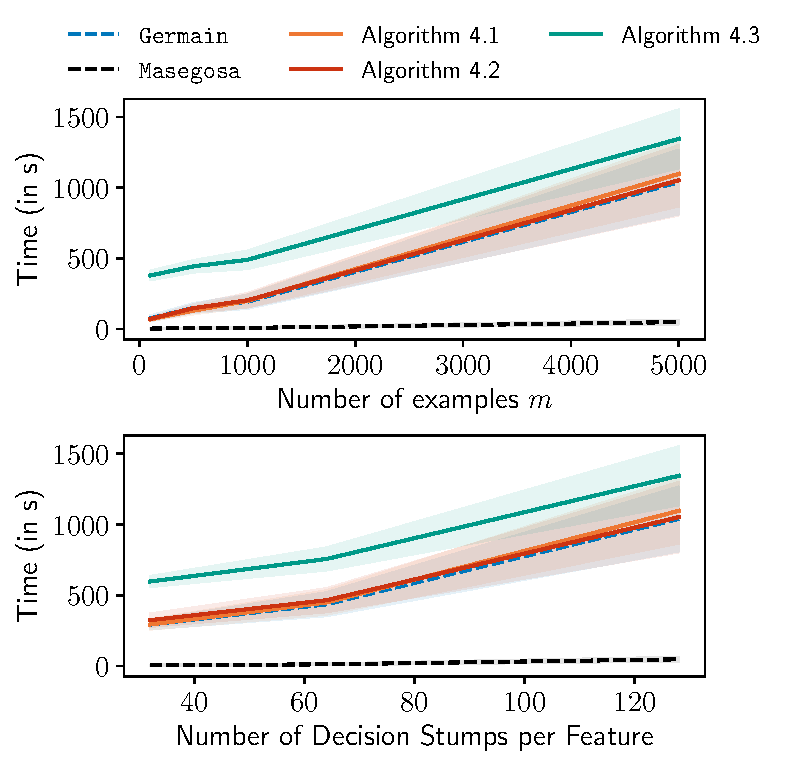
\includegraphics[width=0.9\linewidth]{chapter_4/figures/moons_time.pdf}
    \caption{
    In the top plot represents the evolution of the computation time (in second) with respect to the number of examples $\m$ in moons dataset.
    The bottom plot is the evolution of the computation time in function of the number of decision stumps per feature. 
    For each curve, we plot the mean computation time (the plain line) and the standard deviation (the shadow) over 10 runs.
    }
    \label{chap:mv:fig:moons-time}
\end{figure}

\subsection{Details on the Empirical Joint Error and Disagreement}
\label{ap:mv:sec:joint-disa}

We report in \Cref{chap:mv:fig:cbound-stump-binary-1,chap:mv:fig:cbound-stump-binary-2,chap:mv:fig:cbound-tree-binary-1,chap:mv:fig:cbound-tree-binary-2,chap:mv:fig:cbound-tree-multi-1,chap:mv:fig:cbound-tree-multi-2}, the empirical joint error and disagreement obtained on the different datasets.
These figures illustrate that the solutions found by \Cref{chap:mv:algo:lacasse}, \algomasegosa and \cbboost are similar while \mincq and \algogermain provide usually very different solutions.

\begin{figure}[H]
    \centering
    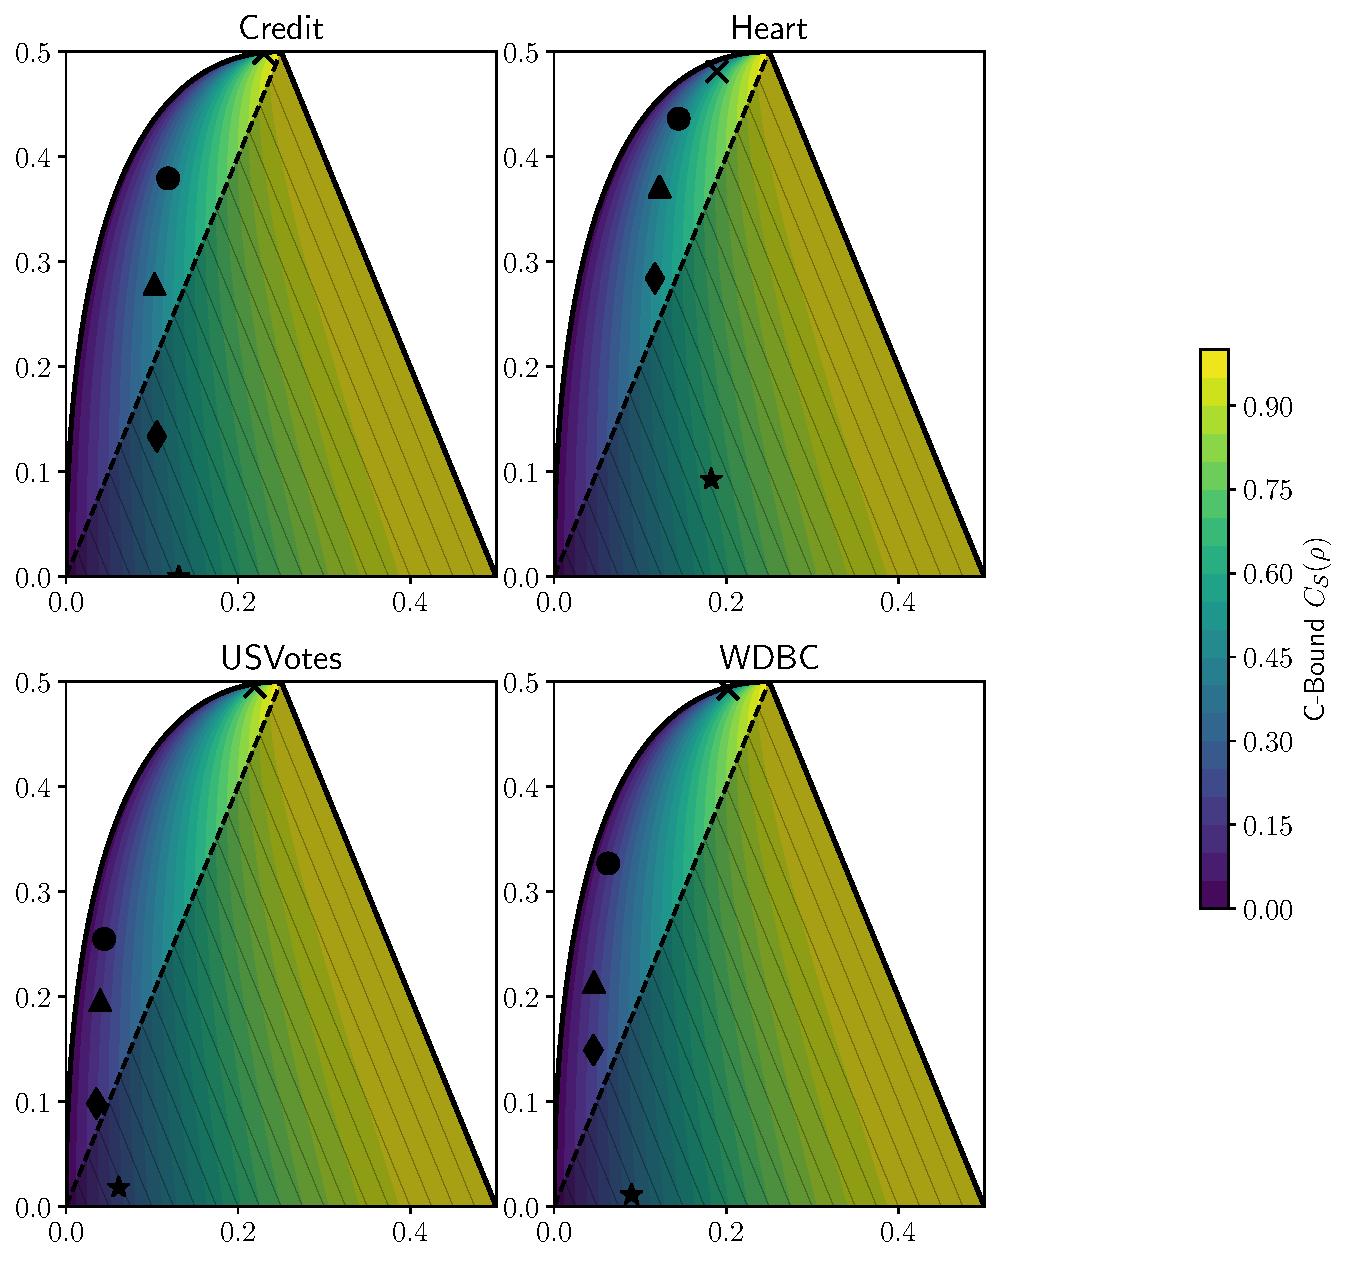
\includegraphics[width=1.0\linewidth]{chapter_4/figures/cbound_stump_binary_1.pdf}
    \caption{
    Representation of all the possible values of the empirical C-Bound $\CBound_{\dS}(\Q)$ in function of the disagreement $d_{\dS}(\Q)$ (y-axis) and joint error $e_{\dS}(\Q)$ (x-axis).
We report the values obtained with the decision stumps in the binary setting by \Cref{chap:mv:algo:lacasse} ($\blacklozenge$), \algomasegosa ($\blacktriangle$), \algogermain~($\bigstar$), \cbboost ($\bullet$), and \mincq ($\boldsymbol{\times}$).
The disagreement and the joint are averaged over the 10 runs.
    }
    \label{chap:mv:fig:cbound-stump-binary-1}
\end{figure}

\begin{figure}
    \centering
    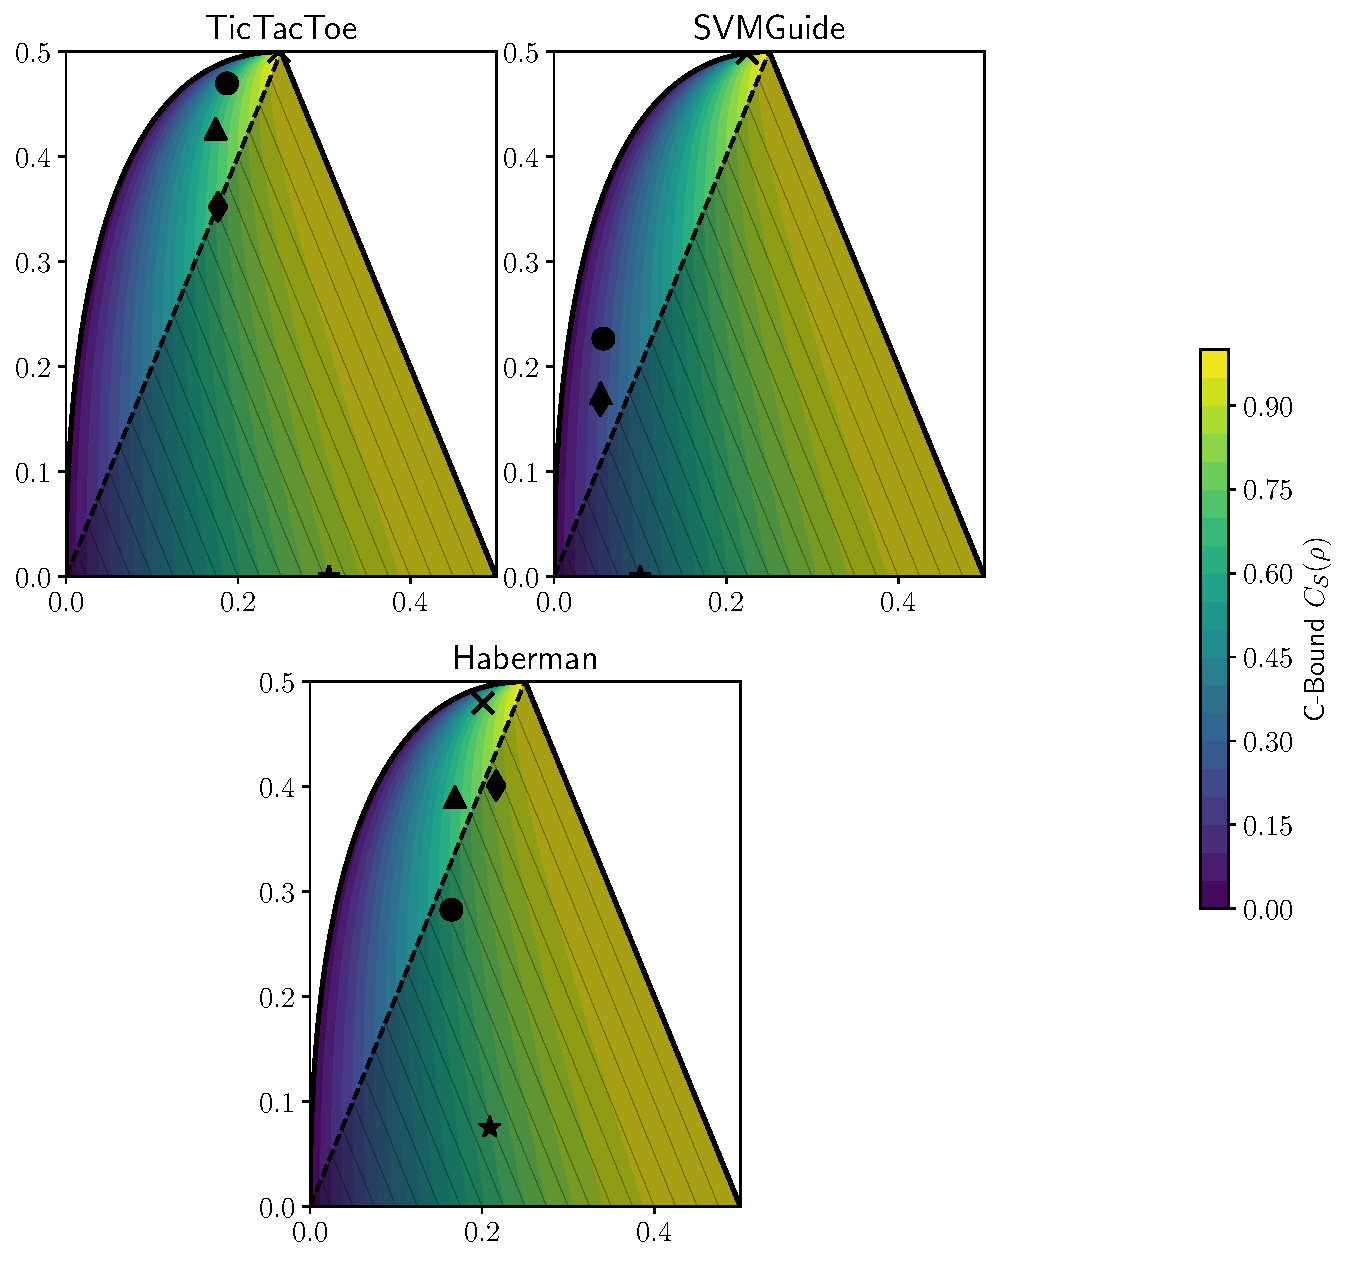
\includegraphics[width=1.0\linewidth]{chapter_4/figures/cbound_stump_binary_2.pdf}
    \caption{
    Representation of all the possible values of the empirical C-Bound $\CBound_{\dS}(\Q)$ in function of the disagreement $d_{\dS}(\Q)$ (y-axis) and joint error $e_{\dS}(\Q)$ (x-axis).
We report the values obtained with the decision stumps in the binary setting by \Cref{chap:mv:algo:lacasse} ($\blacklozenge$), \algomasegosa ($\blacktriangle$), \algogermain~($\bigstar$), \cbboost ($\bullet$), and \mincq ($\boldsymbol{\times}$).
The disagreement and the joint are averaged over the 10 runs.
    }
    \label{chap:mv:fig:cbound-stump-binary-2}
\end{figure}

\begin{figure}
    \centering
    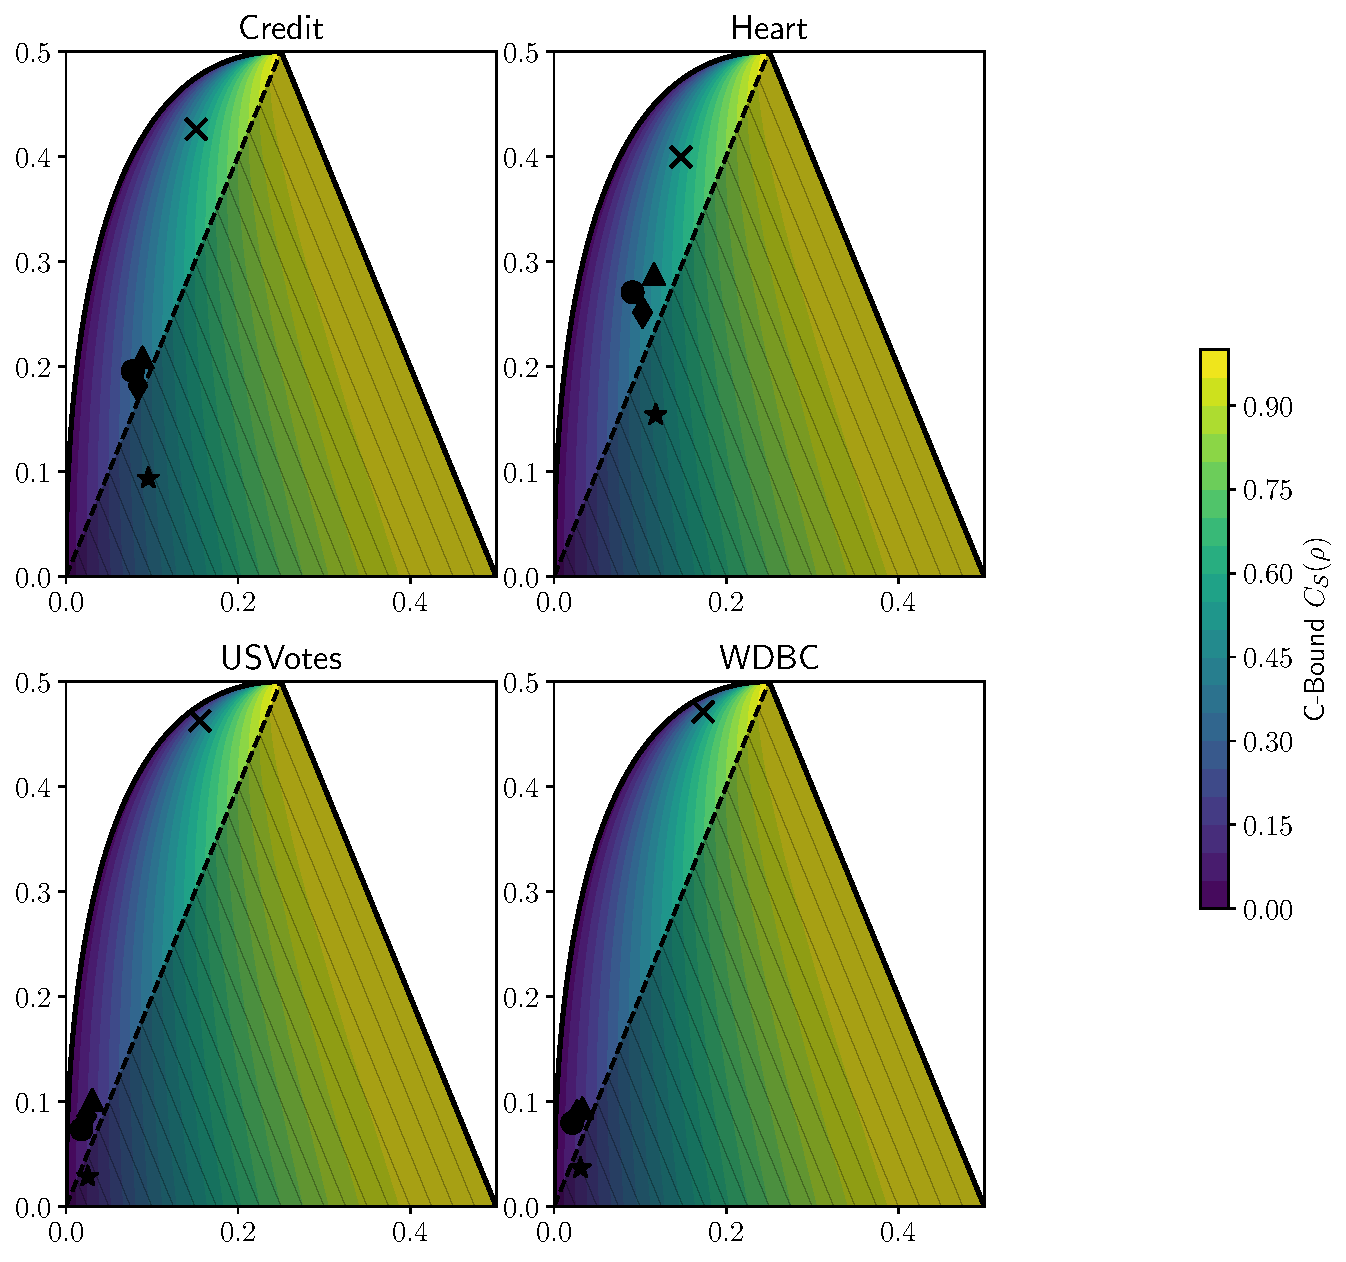
\includegraphics[width=1.0\linewidth]{chapter_4/figures/cbound_tree_binary_1.pdf}
    \caption{
    Representation of all the possible values of the empirical C-Bound $\CBound_{\dS}(\Q)$ in function of the disagreement $d_{\dS}(\Q)$ (y-axis) and joint error $e_{\dS}(\Q)$ (x-axis).
We report the values obtained with the decision trees in the binary setting by \Cref{chap:mv:algo:lacasse} ($\blacklozenge$), \algomasegosa ($\blacktriangle$), \algogermain~($\bigstar$), \cbboost ($\bullet$), and \mincq ($\boldsymbol{\times}$).
The disagreement and the joint are averaged over the 10 runs.
    }
    \label{chap:mv:fig:cbound-tree-binary-1}
\end{figure}

\begin{figure}
    \centering
    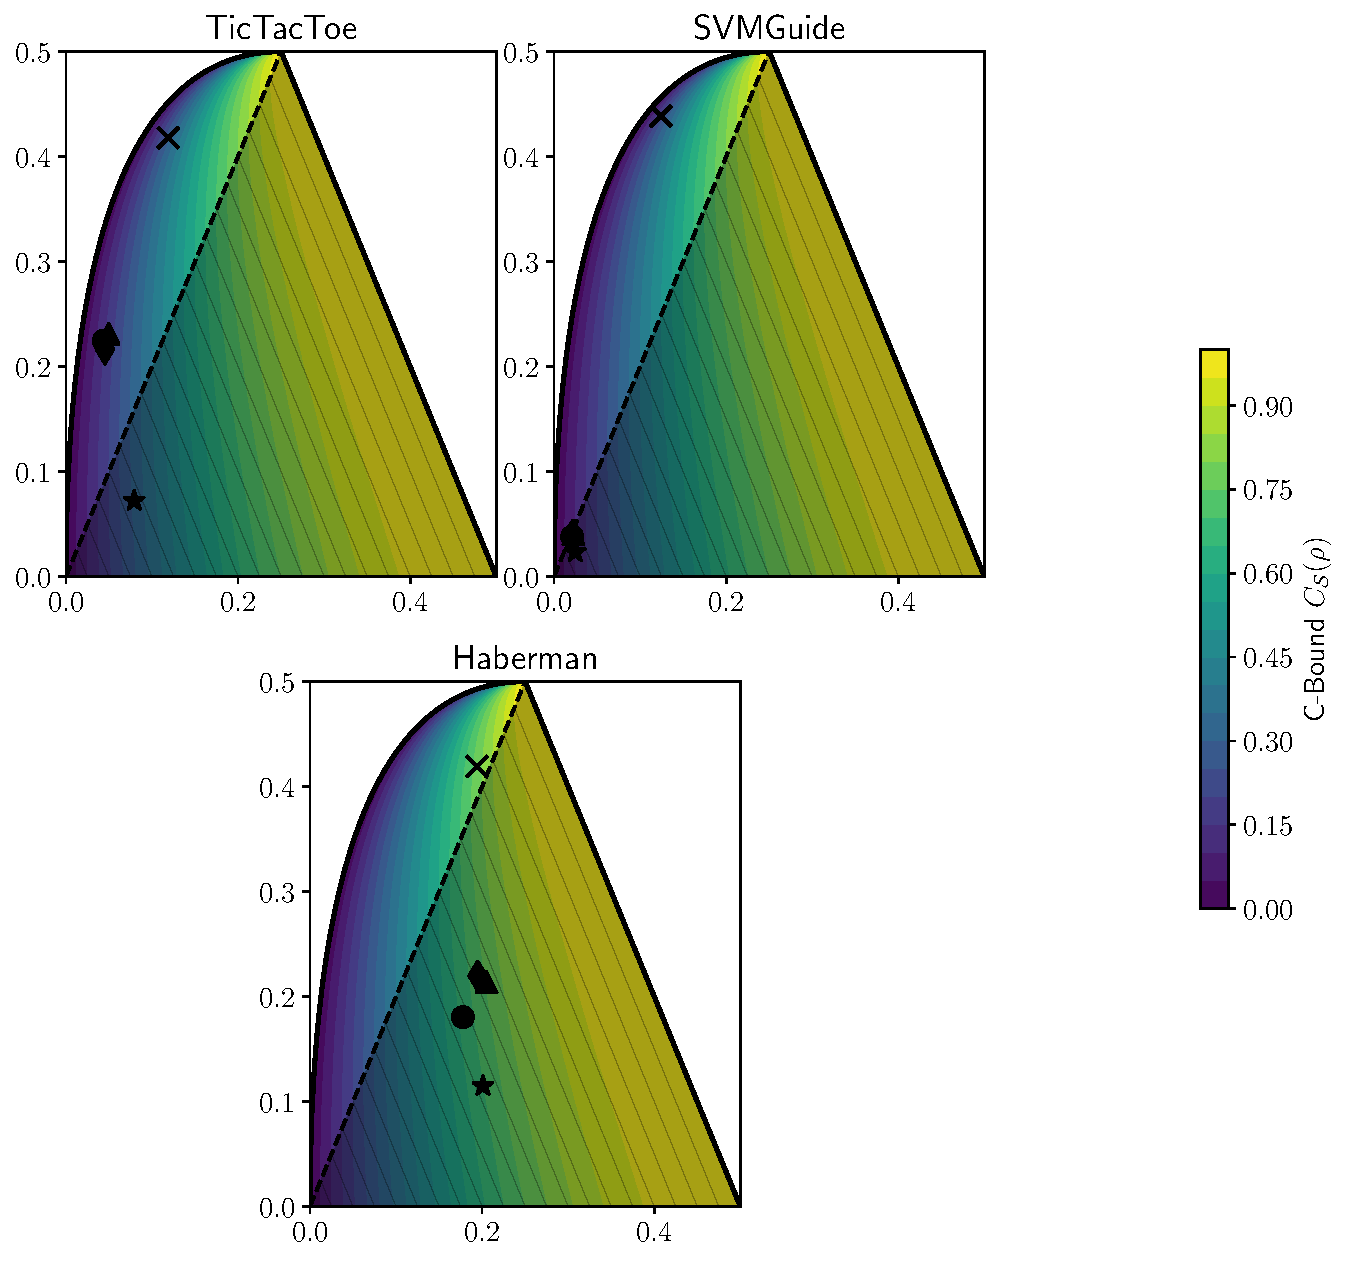
\includegraphics[width=1.0\linewidth]{chapter_4/figures/cbound_tree_binary_2.pdf}
    \caption{
    Representation of all the possible values of the empirical C-Bound $\CBound_{\dS}(\Q)$ in function of the disagreement $d_{\dS}(\Q)$ (y-axis) and joint error $e_{\dS}(\Q)$ (x-axis).
We report the values obtained with the decision trees in the binary setting by \Cref{chap:mv:algo:lacasse} ($\blacklozenge$), \algomasegosa ($\blacktriangle$), \algogermain~($\bigstar$), \cbboost ($\bullet$), and \mincq ($\boldsymbol{\times}$).
The disagreement and the joint are averaged over the 10 runs.
    }
    \label{chap:mv:fig:cbound-tree-binary-2}
\end{figure}

\begin{figure}
    \centering
    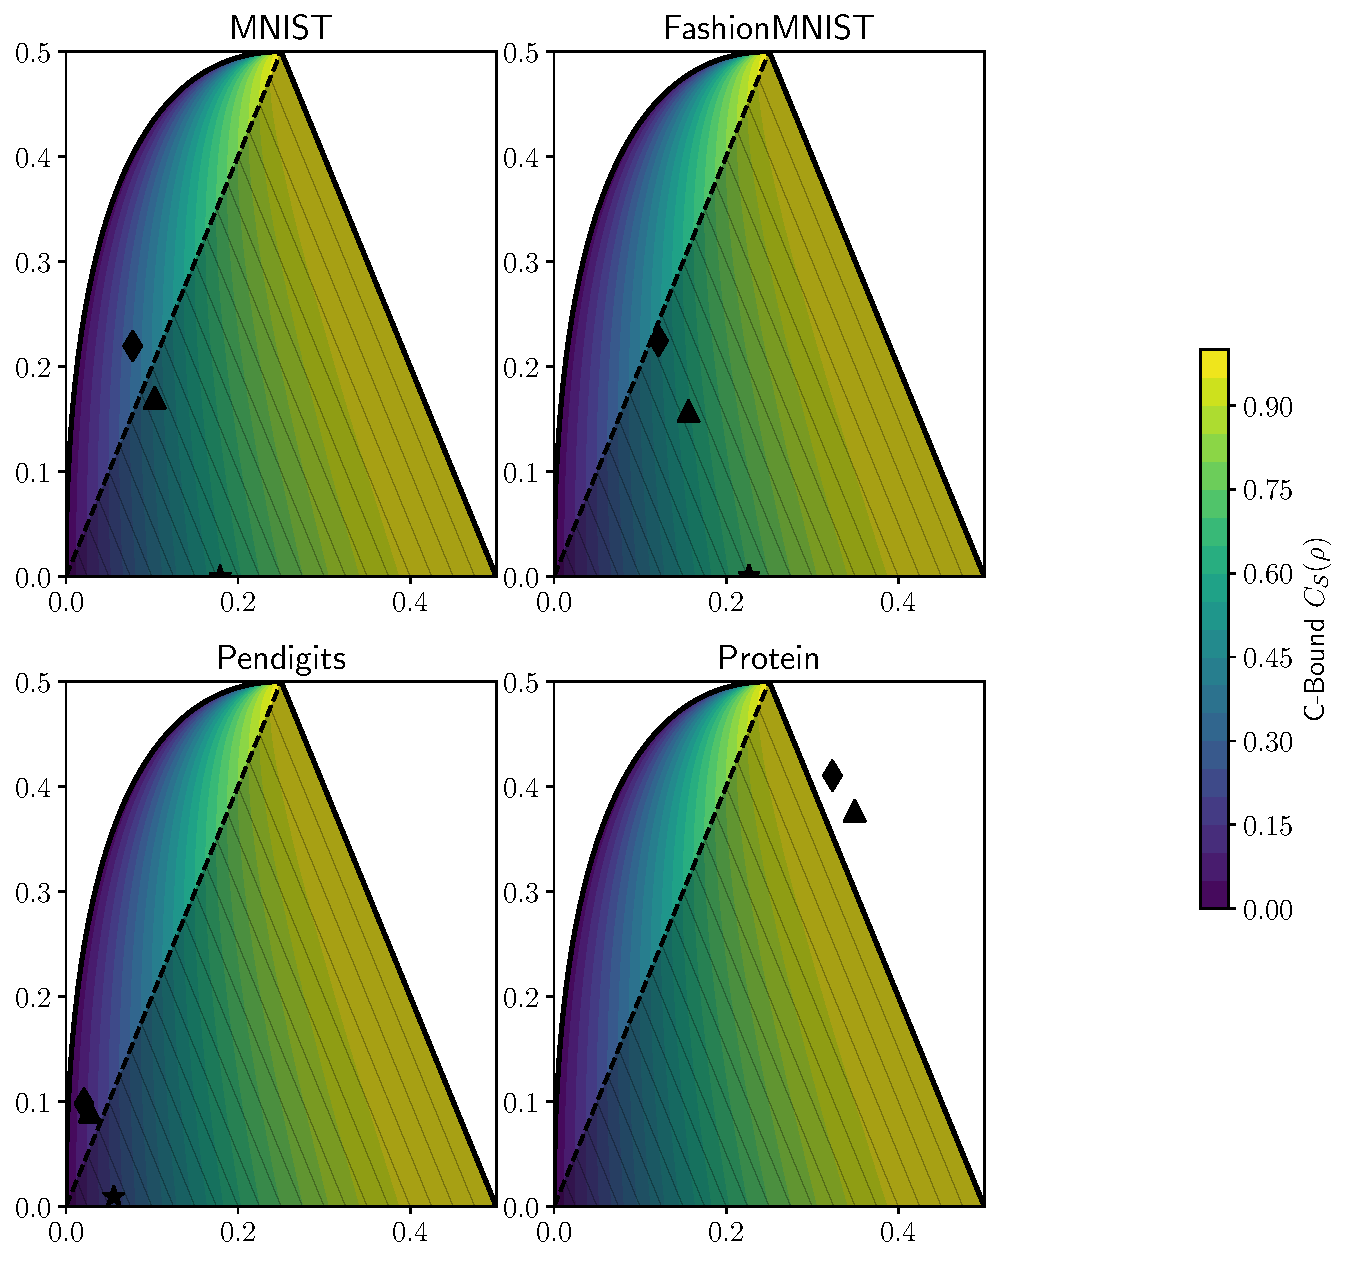
\includegraphics[width=1.0\linewidth]{chapter_4/figures/cbound_tree_multi_1.pdf}
    \caption{
    Representation of all the possible values of the empirical C-Bound $\CBound_{\dS}(\Q)$ in function of the disagreement $d_{\dS}(\Q)$ (y-axis) and joint error $e_{\dS}(\Q)$ (x-axis).
We report the values obtained with the decision trees in the multi-class setting by \Cref{chap:mv:algo:lacasse} ($\blacklozenge$), \algomasegosa ($\blacktriangle$), \algogermain~($\bigstar$).
The disagreement and the joint are averaged over the 10 runs.
    }
    \label{chap:mv:fig:cbound-tree-multi-1}
\end{figure}

\begin{figure}
    \centering
    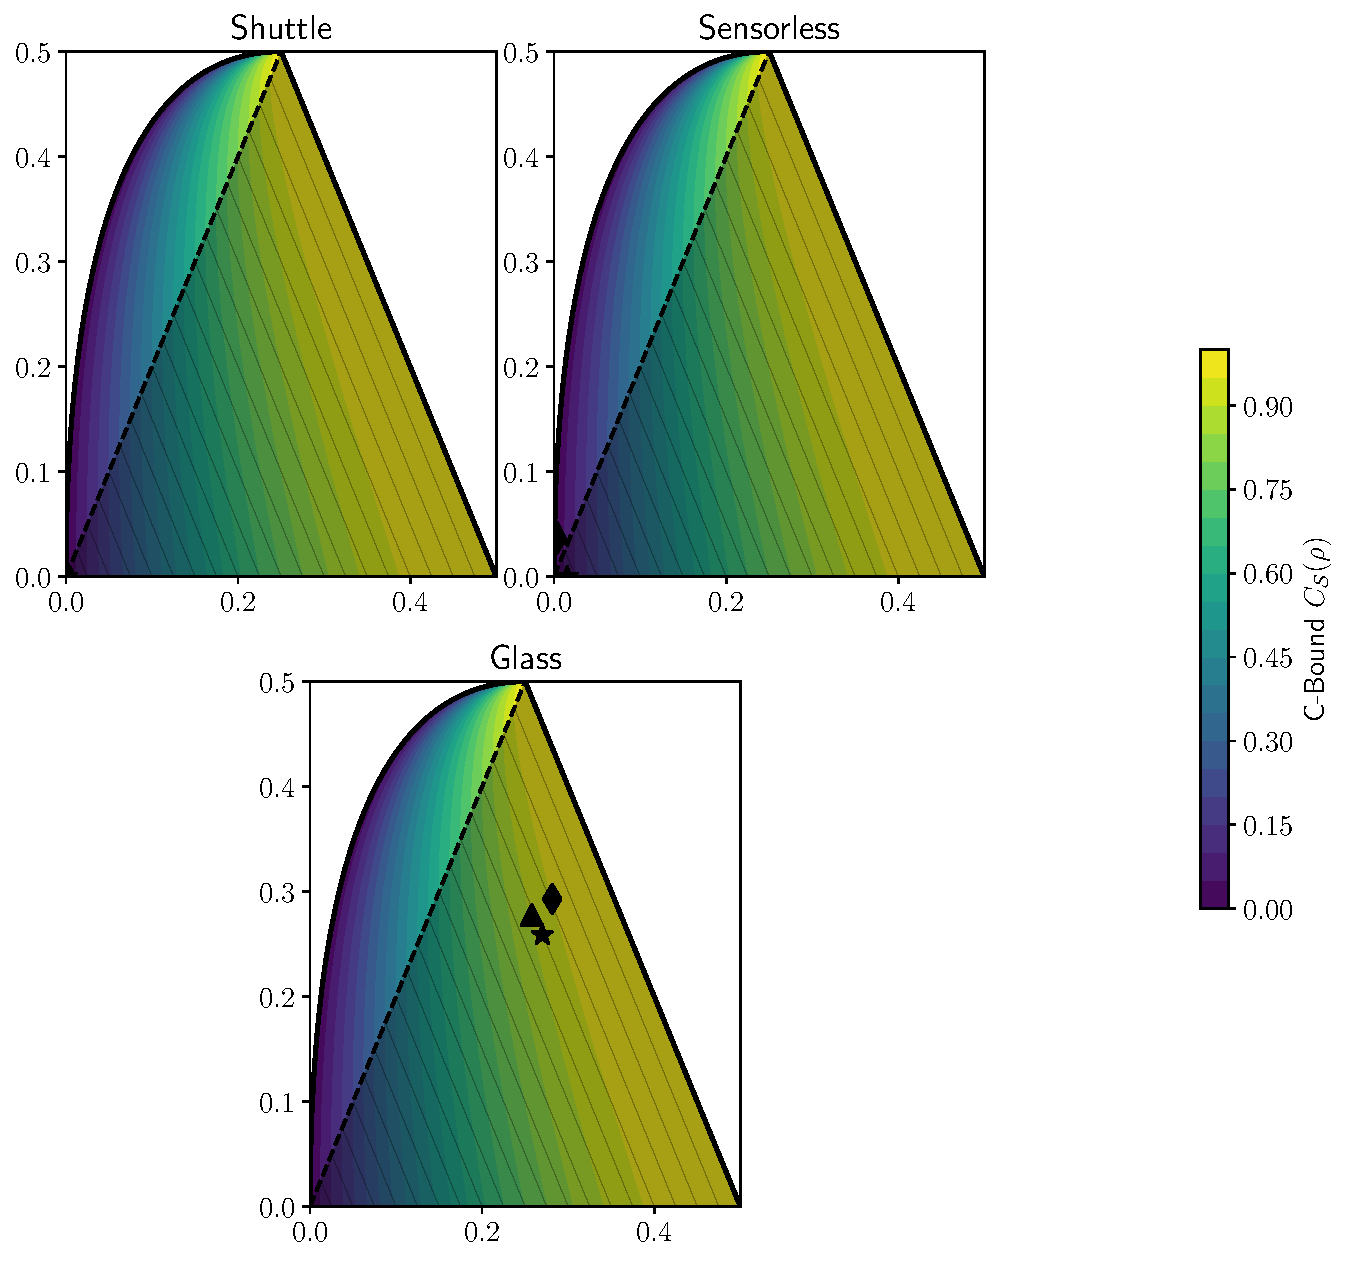
\includegraphics[width=1.0\linewidth]{chapter_4/figures/cbound_tree_multi_2.pdf}
    \caption{
    Representation of all the possible values of the empirical C-Bound $\CBound_{\dS}(\Q)$ in function of the disagreement $d_{\dS}(\Q)$ (y-axis) and joint error $e_{\dS}(\Q)$ (x-axis).
We report the values obtained with the decision trees in the multi-class setting by \Cref{chap:mv:algo:lacasse} ($\blacklozenge$), \algomasegosa ($\blacktriangle$), \algogermain~($\bigstar$).
The disagreement and the joint are averaged over the 10 runs.
    }
    \label{chap:mv:fig:cbound-tree-multi-2}
\end{figure}

\begin{landscape}
\begin{table}[t]
\centering
\caption{
Comparison of the true risks $\Risk_{\dT}(\MVQ)$ and bound values obtained for each algorithm over 10 runs when the voters are decision stumps in the binary setting.
More precisely, we report the mean $\pm$ the standard deviation.
``Bound'' is the mean value of the bound that is optimized, excepted for \mincq and \cbboost for which we report the bound obtained with \Cref{chap:mv:theorem:new-cbound-lacasse} instantiated with the majority vote learned. 
Results in {\bf bold} are the couple ($\Risk_{\dT}(\MVQ)$, Bound) associated to {\bf the lowest risk} value.
{\it Italic} and \underline{underlined} results are the couple  ($\Risk_{\dT}(\MVQ)$, Bound) associated respectively to \textit{the lowest bound} value and \underline{the second lowest bound} values.
}
\begin{subtable}[t]{2.0\textwidth}
\scalebox{0.69}{
\begin{tabular}{l|cc||cc||cc||ccHHHHHH}
\toprule
 & \multicolumn{2}{r}{Algorithm 4.1} & \multicolumn{2}{r}{Algorithm 4.2} & \multicolumn{2}{r}{Algorithm 4.3} & \multicolumn{2}{r}{\algomasegosa} & \multicolumn{2}{r}{\algogermain} & \multicolumn{2}{r}{\cbboost} & \multicolumn{2}{r}{\mincq} \\
 & $\Risk_{\dT}(\MVQ)$ & Bound & $\Risk_{\dT}(\MVQ)$ & Bound & $\Risk_{\dT}(\MVQ)$ & Bound & $\Risk_{\dT}(\MVQ)$ & Bound & $\Risk_{\dT}(\MVQ)$ & Bound & $\Risk_{\dT}(\MVQ)$ & Bound & $\Risk_{\dT}(\MVQ)$ & Bound \\
\midrule
Credit & .141 $\pm$ .014 & .772 $\pm$ .026 & \underline{.141 $\pm$ .014} & \underline{.718 $\pm$ .036} & .141 $\pm$ .014 & .748 $\pm$ .037 & .141 $\pm$ .014 & .784 $\pm$ .047 & \textit{.141 $\pm$ .014} & \textit{.462 $\pm$ .033} & \textbf{.140 $\pm$ .015} & \textbf{.917 $\pm$ .049} & .141 $\pm$ .020 & 1.000 $\pm$ .000 \\
Heart & .252 $\pm$ .034 & .970 $\pm$ .011 & .252 $\pm$ .034 & .960 $\pm$ .013 & \underline{\textbf{.161 $\pm$ .028}} & \underline{\textbf{.937 $\pm$ .017}} & .163 $\pm$ .025 & 1.041 $\pm$ .034 & \textit{.257 $\pm$ .026} & \textit{.796 $\pm$ .036} & .191 $\pm$ .016 & .996 $\pm$ .007 & .185 $\pm$ .017 & 1.000 $\pm$ .000 \\
USVotes & .043 $\pm$ .007 & .657 $\pm$ .016 & \underline{.043 $\pm$ .007} & \underline{.494 $\pm$ .034} & \textbf{.042 $\pm$ .008} & \textbf{.529 $\pm$ .029} & \textbf{.042 $\pm$ .008} & \textbf{.520 $\pm$ .030} & \textit{.068 $\pm$ .040} & \textit{.351 $\pm$ .108} & .043 $\pm$ .007 & .683 $\pm$ .038 & .048 $\pm$ .009 & 1.000 $\pm$ .000 \\
WDBC & .101 $\pm$ .030 & .722 $\pm$ .016 & .115 $\pm$ .031 & .675 $\pm$ .050 & .069 $\pm$ .014 & .578 $\pm$ .024 & \underline{.060 $\pm$ .010} & \underline{.533 $\pm$ .021} & \textit{.105 $\pm$ .023} & \textit{.412 $\pm$ .032} & \textbf{.044 $\pm$ .008} & \textbf{.687 $\pm$ .044} & .044 $\pm$ .013 & 1.000 $\pm$ .000 \\
TicTacToe & .296 $\pm$ .011 & .969 $\pm$ .008 & .296 $\pm$ .011 & .967 $\pm$ .009 & \underline{.303 $\pm$ .015} & \underline{.958 $\pm$ .009} & .272 $\pm$ .024 & 1.021 $\pm$ .016 & \textit{.296 $\pm$ .011} & \textit{.812 $\pm$ .023} & .202 $\pm$ .020 & 1.000 $\pm$ .000 & \textbf{.020 $\pm$ .003} & \textbf{1.000 $\pm$ .000} \\
SVMGuide & .085 $\pm$ .007 & .463 $\pm$ .028 & .085 $\pm$ .007 & .385 $\pm$ .025 & .081 $\pm$ .014 & .325 $\pm$ .011 & \underline{.076 $\pm$ .012} & \underline{.313 $\pm$ .011} & \textit{.102 $\pm$ .035} & \textit{.256 $\pm$ .086} & .068 $\pm$ .012 & .334 $\pm$ .012 & \textbf{.048 $\pm$ .002} & \textbf{1.000 $\pm$ .000} \\
Haberman & .266 $\pm$ .025 & .975 $\pm$ .012 & \underline{.263 $\pm$ .025} & \underline{.968 $\pm$ .015} & .262 $\pm$ .024 & .988 $\pm$ .020 & \textbf{.260 $\pm$ .019} & \textbf{1.207 $\pm$ .050} & \textit{.265 $\pm$ .026} & \textit{.811 $\pm$ .046} & .274 $\pm$ .029 & .988 $\pm$ .011 & .261 $\pm$ .016 & 1.000 $\pm$ .000 \\
\bottomrule
\end{tabular}

}
\end{subtable}
\newline
\vspace*{1cm}
\newline
\begin{subtable}[t]{1.3\textwidth}
\centering
\scalebox{0.69}{
\begin{tabular}{l|HHHHHHHHcc||cc||cc}
\toprule
 & \multicolumn{2}{H}{Algorithm 4.1} & \multicolumn{2}{H}{Algorithm 4.2} & \multicolumn{2}{H}{Algorithm 4.3} & \multicolumn{2}{H}{\algomasegosa} & \multicolumn{2}{c}{\algogermain} & \multicolumn{2}{c}{\cbboost} & \multicolumn{2}{c}{\mincq} \\
 & $\Risk_{\dT}(\MVQ)$ & Bound & $\Risk_{\dT}(\MVQ)$ & Bound & $\Risk_{\dT}(\MVQ)$ & Bound & $\Risk_{\dT}(\MVQ)$ & Bound & $\Risk_{\dT}(\MVQ)$ & Bound & $\Risk_{\dT}(\MVQ)$ & Bound & $\Risk_{\dT}(\MVQ)$ & Bound \\
\midrule
Credit & .141 $\pm$ .014 & .772 $\pm$ .026 & \underline{.141 $\pm$ .014} & \underline{.718 $\pm$ .036} & .141 $\pm$ .014 & .748 $\pm$ .037 & .141 $\pm$ .014 & .784 $\pm$ .047 & \textit{.141 $\pm$ .014} & \textit{.462 $\pm$ .033} & \textbf{.140 $\pm$ .015} & \textbf{.917 $\pm$ .049} & .141 $\pm$ .020 & 1.000 $\pm$ .000 \\
Heart & .252 $\pm$ .034 & .970 $\pm$ .011 & .252 $\pm$ .034 & .960 $\pm$ .013 & \underline{\textbf{.161 $\pm$ .028}} & \underline{\textbf{.937 $\pm$ .017}} & .163 $\pm$ .025 & 1.041 $\pm$ .034 & \textit{.257 $\pm$ .026} & \textit{.796 $\pm$ .036} & .191 $\pm$ .016 & .996 $\pm$ .007 & .185 $\pm$ .017 & 1.000 $\pm$ .000 \\
USVotes & .043 $\pm$ .007 & .657 $\pm$ .016 & \underline{.043 $\pm$ .007} & \underline{.494 $\pm$ .034} & \textbf{.042 $\pm$ .008} & \textbf{.529 $\pm$ .029} & \textbf{.042 $\pm$ .008} & \textbf{.520 $\pm$ .030} & \textit{.068 $\pm$ .040} & \textit{.351 $\pm$ .108} & .043 $\pm$ .007 & .683 $\pm$ .038 & .048 $\pm$ .009 & 1.000 $\pm$ .000 \\
WDBC & .101 $\pm$ .030 & .722 $\pm$ .016 & .115 $\pm$ .031 & .675 $\pm$ .050 & .069 $\pm$ .014 & .578 $\pm$ .024 & \underline{.060 $\pm$ .010} & \underline{.533 $\pm$ .021} & \textit{.105 $\pm$ .023} & \textit{.412 $\pm$ .032} & \textbf{.044 $\pm$ .008} & \textbf{.687 $\pm$ .044} & .044 $\pm$ .013 & 1.000 $\pm$ .000 \\
TicTacToe & .296 $\pm$ .011 & .969 $\pm$ .008 & .296 $\pm$ .011 & .967 $\pm$ .009 & \underline{.303 $\pm$ .015} & \underline{.958 $\pm$ .009} & .272 $\pm$ .024 & 1.021 $\pm$ .016 & \textit{.296 $\pm$ .011} & \textit{.812 $\pm$ .023} & .202 $\pm$ .020 & 1.000 $\pm$ .000 & \textbf{.020 $\pm$ .003} & \textbf{1.000 $\pm$ .000} \\
SVMGuide & .085 $\pm$ .007 & .463 $\pm$ .028 & .085 $\pm$ .007 & .385 $\pm$ .025 & .081 $\pm$ .014 & .325 $\pm$ .011 & \underline{.076 $\pm$ .012} & \underline{.313 $\pm$ .011} & \textit{.102 $\pm$ .035} & \textit{.256 $\pm$ .086} & .068 $\pm$ .012 & .334 $\pm$ .012 & \textbf{.048 $\pm$ .002} & \textbf{1.000 $\pm$ .000} \\
Haberman & .266 $\pm$ .025 & .975 $\pm$ .012 & \underline{.263 $\pm$ .025} & \underline{.968 $\pm$ .015} & .262 $\pm$ .024 & .988 $\pm$ .020 & \textbf{.260 $\pm$ .019} & \textbf{1.207 $\pm$ .050} & \textit{.265 $\pm$ .026} & \textit{.811 $\pm$ .046} & .274 $\pm$ .029 & .988 $\pm$ .011 & .261 $\pm$ .016 & 1.000 $\pm$ .000 \\
\bottomrule
\end{tabular}

}
\end{subtable}
\label{chap:mv:table:stump-binary}
\end{table}
\end{landscape}

\begin{landscape}
\begin{table}[t]
\centering
\caption{
Comparison of the true risks $\Risk_{\dT}(\MVQ)$ and bound values obtained for each algorithm over 10 runs when the voters are decision trees in the binary setting.
More precisely, we report the mean $\pm$ the standard deviation.
``Bound'' is the mean value of the bound that is optimized, excepted for \mincq and \cbboost for which we report the bound obtained with \Cref{chap:mv:theorem:new-cbound-lacasse} instantiated with the majority vote learned. 
Results in {\bf bold} are the couple ($\Risk_{\dT}(\MVQ)$, Bound) associated to {\bf the lowest risk} value.
{\it Italic} and \underline{underlined} results are the couple  ($\Risk_{\dT}(\MVQ)$, Bound) associated respectively to \textit{the lowest bound} value and \underline{the second lowest bound} values.
}
\begin{subtable}[t]{2.0\textwidth}
\scalebox{0.69}{
\begin{tabular}{l|cc||cc||cc||ccHHHHHH}
\toprule
 & \multicolumn{2}{c}{Algorithm 4.1} & \multicolumn{2}{c}{Algorithm 4.2} & \multicolumn{2}{c}{Algorithm 4.3} & \multicolumn{2}{c}{\algomasegosa} & \multicolumn{2}{H}{\algogermain} & \multicolumn{2}{H}{\cbboost} & \multicolumn{2}{H}{\mincq} \\
 & $\Risk_{\dT}(\MVQ)$ & Bound & $\Risk_{\dT}(\MVQ)$ & Bound & $\Risk_{\dT}(\MVQ)$ & Bound & $\Risk_{\dT}(\MVQ)$ & Bound & $\Risk_{\dT}(\MVQ)$ & Bound & $\Risk_{\dT}(\MVQ)$ & Bound & $\Risk_{\dT}(\MVQ)$ & Bound \\
\midrule
Credit & .156 $\pm$ .018 & .861 $\pm$ .034 & .154 $\pm$ .021 & .807 $\pm$ .048 & \underline{.142 $\pm$ .015} & \underline{.744 $\pm$ .057} & \textbf{.138 $\pm$ .015} & \textbf{.775 $\pm$ .081} & \textit{.167 $\pm$ .023} & \textit{.564 $\pm$ .059} & .147 $\pm$ .017 & .772 $\pm$ .054 & .140 $\pm$ .021 & .981 $\pm$ .025 \\
Heart & .230 $\pm$ .027 & .984 $\pm$ .011 & .228 $\pm$ .025 & .976 $\pm$ .018 & \underline{\textbf{.210 $\pm$ .026}} & \underline{\textbf{.956 $\pm$ .025}} & .213 $\pm$ .026 & 1.161 $\pm$ .076 & \textit{.234 $\pm$ .022} & \textit{.840 $\pm$ .059} & .222 $\pm$ .026 & .972 $\pm$ .019 & .222 $\pm$ .029 & 1.000 $\pm$ .000 \\
USVotes & .053 $\pm$ .011 & .738 $\pm$ .031 & .057 $\pm$ .012 & .571 $\pm$ .067 & \textbf{.046 $\pm$ .014} & \textbf{.523 $\pm$ .059} & \underline{.051 $\pm$ .023} & \underline{.513 $\pm$ .069} & \textit{.056 $\pm$ .012} & \textit{.334 $\pm$ .050} & .048 $\pm$ .019 & .578 $\pm$ .050 & .053 $\pm$ .010 & .989 $\pm$ .032 \\
WDBC & .054 $\pm$ .010 & .705 $\pm$ .022 & .061 $\pm$ .010 & .554 $\pm$ .041 & .045 $\pm$ .007 & .485 $\pm$ .042 & \underline{.049 $\pm$ .011} & \underline{.471 $\pm$ .050} & \textit{.063 $\pm$ .010} & \textit{.324 $\pm$ .033} & \textbf{.044 $\pm$ .012} & \textbf{.525 $\pm$ .042} & .054 $\pm$ .013 & .984 $\pm$ .041 \\
TicTacToe & .056 $\pm$ .010 & .776 $\pm$ .025 & .078 $\pm$ .023 & .685 $\pm$ .047 & \textbf{.048 $\pm$ .013} & \textbf{.530 $\pm$ .052} & \underline{.050 $\pm$ .010} & \underline{.493 $\pm$ .054} & \textit{.127 $\pm$ .025} & \textit{.457 $\pm$ .047} & .049 $\pm$ .014 & .545 $\pm$ .052 & .049 $\pm$ .013 & .901 $\pm$ .080 \\
SVMGuide & .033 $\pm$ .002 & .340 $\pm$ .011 & .033 $\pm$ .001 & .213 $\pm$ .012 & .032 $\pm$ .002 & .177 $\pm$ .012 & \underline{\textbf{.032 $\pm$ .002}} & \underline{\textbf{.165 $\pm$ .012}} & \textit{.038 $\pm$ .005} & \textit{.123 $\pm$ .008} & .033 $\pm$ .002 & .183 $\pm$ .012 & .033 $\pm$ .002 & .660 $\pm$ .185 \\
Haberman & .307 $\pm$ .031 & .998 $\pm$ .004 & .307 $\pm$ .030 & .997 $\pm$ .006 & \underline{.295 $\pm$ .025} & \underline{.997 $\pm$ .006} & \textbf{.294 $\pm$ .018} & \textbf{1.586 $\pm$ .113} & \textit{.306 $\pm$ .030} & \textit{.970 $\pm$ .058} & .295 $\pm$ .024 & .999 $\pm$ .002 & .296 $\pm$ .016 & 1.000 $\pm$ .000 \\
\bottomrule
\end{tabular}

}
\end{subtable}
\newline
\vspace*{1cm}
\newline
\begin{subtable}[t]{1.3\textwidth}
\centering
\scalebox{0.69}{
\begin{tabular}{l|HHHHHHHHcc||cc||cc}
\toprule
 & \multicolumn{2}{r}{Algorithm 4.1} & \multicolumn{2}{r}{Algorithm 4.2} & \multicolumn{2}{r}{Algorithm 4.3} & \multicolumn{2}{r}{\algomasegosa} & \multicolumn{2}{r}{\algogermain} & \multicolumn{2}{r}{\cbboost} & \multicolumn{2}{r}{\mincq} \\
 & $\Risk_{\dT}(\MVQ)$ & Bound & $\Risk_{\dT}(\MVQ)$ & Bound & $\Risk_{\dT}(\MVQ)$ & Bound & $\Risk_{\dT}(\MVQ)$ & Bound & $\Risk_{\dT}(\MVQ)$ & Bound & $\Risk_{\dT}(\MVQ)$ & Bound & $\Risk_{\dT}(\MVQ)$ & Bound \\
\midrule
Credit & .156 $\pm$ .018 & .861 $\pm$ .034 & .154 $\pm$ .021 & .807 $\pm$ .048 & \underline{.142 $\pm$ .015} & \underline{.744 $\pm$ .057} & \textbf{.138 $\pm$ .015} & \textbf{.775 $\pm$ .081} & \textit{.167 $\pm$ .023} & \textit{.564 $\pm$ .059} & .147 $\pm$ .017 & .772 $\pm$ .054 & .140 $\pm$ .021 & .981 $\pm$ .025 \\
Heart & .230 $\pm$ .027 & .984 $\pm$ .011 & .228 $\pm$ .025 & .976 $\pm$ .018 & \underline{\textbf{.210 $\pm$ .026}} & \underline{\textbf{.956 $\pm$ .025}} & .213 $\pm$ .026 & 1.161 $\pm$ .076 & \textit{.234 $\pm$ .022} & \textit{.840 $\pm$ .059} & .222 $\pm$ .026 & .972 $\pm$ .019 & .222 $\pm$ .029 & 1.000 $\pm$ .000 \\
USVotes & .053 $\pm$ .011 & .738 $\pm$ .031 & .057 $\pm$ .012 & .571 $\pm$ .067 & \textbf{.046 $\pm$ .014} & \textbf{.523 $\pm$ .059} & \underline{.051 $\pm$ .023} & \underline{.513 $\pm$ .069} & \textit{.056 $\pm$ .012} & \textit{.334 $\pm$ .050} & .048 $\pm$ .019 & .578 $\pm$ .050 & .053 $\pm$ .010 & .989 $\pm$ .032 \\
WDBC & .054 $\pm$ .010 & .705 $\pm$ .022 & .061 $\pm$ .010 & .554 $\pm$ .041 & .045 $\pm$ .007 & .485 $\pm$ .042 & \underline{.049 $\pm$ .011} & \underline{.471 $\pm$ .050} & \textit{.063 $\pm$ .010} & \textit{.324 $\pm$ .033} & \textbf{.044 $\pm$ .012} & \textbf{.525 $\pm$ .042} & .054 $\pm$ .013 & .984 $\pm$ .041 \\
TicTacToe & .056 $\pm$ .010 & .776 $\pm$ .025 & .078 $\pm$ .023 & .685 $\pm$ .047 & \textbf{.048 $\pm$ .013} & \textbf{.530 $\pm$ .052} & \underline{.050 $\pm$ .010} & \underline{.493 $\pm$ .054} & \textit{.127 $\pm$ .025} & \textit{.457 $\pm$ .047} & .049 $\pm$ .014 & .545 $\pm$ .052 & .049 $\pm$ .013 & .901 $\pm$ .080 \\
SVMGuide & .033 $\pm$ .002 & .340 $\pm$ .011 & .033 $\pm$ .001 & .213 $\pm$ .012 & .032 $\pm$ .002 & .177 $\pm$ .012 & \underline{\textbf{.032 $\pm$ .002}} & \underline{\textbf{.165 $\pm$ .012}} & \textit{.038 $\pm$ .005} & \textit{.123 $\pm$ .008} & .033 $\pm$ .002 & .183 $\pm$ .012 & .033 $\pm$ .002 & .660 $\pm$ .185 \\
Haberman & .307 $\pm$ .031 & .998 $\pm$ .004 & .307 $\pm$ .030 & .997 $\pm$ .006 & \underline{.295 $\pm$ .025} & \underline{.997 $\pm$ .006} & \textbf{.294 $\pm$ .018} & \textbf{1.586 $\pm$ .113} & \textit{.306 $\pm$ .030} & \textit{.970 $\pm$ .058} & .295 $\pm$ .024 & .999 $\pm$ .002 & .296 $\pm$ .016 & 1.000 $\pm$ .000 \\
\bottomrule
\end{tabular}

}
\end{subtable}
\label{chap:mv:table:tree-binary} 
\end{table}
\end{landscape}

\begin{landscape}
\begin{table}[t]
\centering
\caption{
Comparison of the true risks $\Risk_{\dT}(\MVQ)$ and bound values obtained for each algorithm over 10 runs when the voters are decision trees in the multi-class setting.
More precisely, we report the mean $\pm$ the standard deviation.
Results in {\bf bold} are the couple ($\Risk_{\dT}(\MVQ)$, Bound) associated to {\bf the lowest risk} value.
{\it Italic} and \underline{underlined} results are the couple  ($\Risk_{\dT}(\MVQ)$, Bound) associated respectively to \textit{the lowest bound} value and \underline{the second lowest bound} values.
}
\begin{subtable}[t]{1.0\textwidth}
\scalebox{0.69}{
\begin{tabular}{l|cc||cc||ccHHHH}
\toprule
 & \multicolumn{2}{c}{Algorithm 4.1} & \multicolumn{2}{c}{Algorithm 4.2} & \multicolumn{2}{c}{Algorithm 4.3} & \multicolumn{2}{H}{\algomasegosa} & \multicolumn{2}{H}{\algogermain} \\
 & $\Risk_{\dT}(\MVQ)$ & Bound & $\Risk_{\dT}(\MVQ)$ & Bound & $\Risk_{\dT}(\MVQ)$ & Bound & $\Risk_{\dT}(\MVQ)$ & Bound & $\Risk_{\dT}(\MVQ)$ & Bound \\
\midrule
MNIST & \textbf{.034 $\pm$ .002} & \textbf{.387 $\pm$ .003} & \underline{.034 $\pm$ .002} & \underline{.371 $\pm$ .003} & \textit{.034 $\pm$ .002} & \textit{.340 $\pm$ .004} & .095 $\pm$ .037 & .451 $\pm$ .062 & .180 $\pm$ .005 & .382 $\pm$ .003 \\
FashionMNIST & \textbf{.121 $\pm$ .004} & \textbf{.554 $\pm$ .003} & .121 $\pm$ .004 & .544 $\pm$ .003 & \underline{.121 $\pm$ .004} & \underline{.523 $\pm$ .003} & .195 $\pm$ .022 & .672 $\pm$ .070 & \textit{.231 $\pm$ .004} & \textit{.479 $\pm$ .002} \\
Pendigits & .015 $\pm$ .007 & .283 $\pm$ .007 & .015 $\pm$ .007 & .197 $\pm$ .009 & \textbf{\textit{.015 $\pm$ .007}} & \textbf{\textit{.137 $\pm$ .009}} & .027 $\pm$ .017 & .168 $\pm$ .030 & \underline{.064 $\pm$ .022} & \underline{.163 $\pm$ .010} \\
Protein & \textit{.467 $\pm$ .060} & \textit{1.000 $\pm$ .000} & \textit{.462 $\pm$ .057} & \textit{1.000 $\pm$ .000} & \textbf{\textit{.419 $\pm$ .038}} & \textbf{\textit{1.000 $\pm$ .000}} & .460 $\pm$ .025 & 1.503 $\pm$ .047 & \underline{.529 $\pm$ .003} & \underline{1.098 $\pm$ .006} \\
Shuttle & .000 $\pm$ .000 & .061 $\pm$ .001 & .000 $\pm$ .000 & .006 $\pm$ .001 & \textbf{.000 $\pm$ .000} & \textbf{.005 $\pm$ .000} & \underline{.000 $\pm$ .000} & \underline{.005 $\pm$ .001} & \textit{.001 $\pm$ .000} & \textit{.003 $\pm$ .001} \\
Sensorless & .002 $\pm$ .001 & .097 $\pm$ .001 & .002 $\pm$ .000 & .040 $\pm$ .001 & \textbf{\textit{.001 $\pm$ .000}} & \textbf{\textit{.022 $\pm$ .001}} & \underline{.002 $\pm$ .001} & \underline{.025 $\pm$ .001} & .015 $\pm$ .001 & .040 $\pm$ .002 \\
Glass & \underline{.328 $\pm$ .058} & \underline{1.000 $\pm$ .000} & \underline{.327 $\pm$ .058} & \underline{1.000 $\pm$ .000} & \textit{.328 $\pm$ .060} & \textit{1.000 $\pm$ .000} & \textbf{.324 $\pm$ .056} & \textbf{1.978 $\pm$ .140} & .327 $\pm$ .058 & 1.263 $\pm$ .081 \\
\bottomrule
\end{tabular}

}
\end{subtable}
\newline
\vspace*{1 cm}
\newline
\begin{subtable}[t]{1.0\textwidth}
\centering
\scalebox{0.69}{
\begin{tabular}{l|HHHHHHcccc}
\toprule
 & \multicolumn{2}{H}{Algorithm 4.1} & \multicolumn{2}{H}{Algorithm 4.2} & \multicolumn{2}{H}{Algorithm 4.3} & \multicolumn{2}{c}{\algomasegosa} & \multicolumn{2}{c}{\algogermain} \\
 & $\Risk_{\dT}(\MVQ)$ & Bound & $\Risk_{\dT}(\MVQ)$ & Bound & $\Risk_{\dT}(\MVQ)$ & Bound & $\Risk_{\dT}(\MVQ)$ & Bound & $\Risk_{\dT}(\MVQ)$ & Bound \\
\midrule
MNIST & \textbf{.034 $\pm$ .002} & \textbf{.387 $\pm$ .003} & \underline{.034 $\pm$ .002} & \underline{.371 $\pm$ .003} & \textit{.034 $\pm$ .002} & \textit{.340 $\pm$ .004} & .095 $\pm$ .037 & .451 $\pm$ .062 & .180 $\pm$ .005 & .382 $\pm$ .003 \\
FashionMNIST & \textbf{.121 $\pm$ .004} & \textbf{.554 $\pm$ .003} & .121 $\pm$ .004 & .544 $\pm$ .003 & \underline{.121 $\pm$ .004} & \underline{.523 $\pm$ .003} & .195 $\pm$ .022 & .672 $\pm$ .070 & \textit{.231 $\pm$ .004} & \textit{.479 $\pm$ .002} \\
Pendigits & .015 $\pm$ .007 & .283 $\pm$ .007 & .015 $\pm$ .007 & .197 $\pm$ .009 & \textbf{\textit{.015 $\pm$ .007}} & \textbf{\textit{.137 $\pm$ .009}} & .027 $\pm$ .017 & .168 $\pm$ .030 & \underline{.064 $\pm$ .022} & \underline{.163 $\pm$ .010} \\
Protein & \textit{.467 $\pm$ .060} & \textit{1.000 $\pm$ .000} & \textit{.462 $\pm$ .057} & \textit{1.000 $\pm$ .000} & \textbf{\textit{.419 $\pm$ .038}} & \textbf{\textit{1.000 $\pm$ .000}} & .460 $\pm$ .025 & 1.503 $\pm$ .047 & \underline{.529 $\pm$ .003} & \underline{1.098 $\pm$ .006} \\
Shuttle & .000 $\pm$ .000 & .061 $\pm$ .001 & .000 $\pm$ .000 & .006 $\pm$ .001 & \textbf{.000 $\pm$ .000} & \textbf{.005 $\pm$ .000} & \underline{.000 $\pm$ .000} & \underline{.005 $\pm$ .001} & \textit{.001 $\pm$ .000} & \textit{.003 $\pm$ .001} \\
Sensorless & .002 $\pm$ .001 & .097 $\pm$ .001 & .002 $\pm$ .000 & .040 $\pm$ .001 & \textbf{\textit{.001 $\pm$ .000}} & \textbf{\textit{.022 $\pm$ .001}} & \underline{.002 $\pm$ .001} & \underline{.025 $\pm$ .001} & .015 $\pm$ .001 & .040 $\pm$ .002 \\
Glass & \underline{.328 $\pm$ .058} & \underline{1.000 $\pm$ .000} & \underline{.327 $\pm$ .058} & \underline{1.000 $\pm$ .000} & \textit{.328 $\pm$ .060} & \textit{1.000 $\pm$ .000} & \textbf{.324 $\pm$ .056} & \textbf{1.978 $\pm$ .140} & .327 $\pm$ .058 & 1.263 $\pm$ .081 \\
\bottomrule
\end{tabular}

}
\end{subtable}
\label{chap:mv:table:tree-multi}
\end{table}
\end{landscape}
\end{noaddcontents}